\documentclass{article}
\usepackage{graphicx} %package to manage images
\usepackage[utf8]{inputenc}
\usepackage[a4paper, total={6in, 8in}]{geometry}
\usepackage{xurl}
\usepackage{hyperref}
\usepackage{float}
\title{Relatório 21 \\ Permutation test}
\author{Pedro A. S. O. Neto}
\date{Março, 2023}

\begin{document}

\maketitle

\section{Justificativa}

Após o processamento de dados e a aplicação de todos os filtros (descritos no Report 20), o $N$ de TEA = 18, e não TEA = 425.
Como forma de testar algumas estatísticas (i.e, proporção de fixações e números de alternâncias), decidimos utilizar um teste de permutação.

O procedimento estatístico é o seguinte:
\begin{itemize}
  \item Separa-se os participantes TEA de TD.
  \item Coleta-se um sub-sample da amostra total de participantes TD. O tamanho do sample é igual ao numero de participantes TEA (neste caso, 18).
  \item Computa-se a estatística de interesse para esse sample.
  \item Repete-se este processo N vezes, com reposição dos participantes retirados em cada sub-sample (o mesmo participante pode ser sampleado mais de uma vez).
\end{itemize}

Ao final deste processo, temos uma distribuição de sample da estatística de interesse. Então olhamos novamente para as estatísticas do sample de TEA, e computamos a probabilidade deste sample ter vindo da mesma população que os TD ($p-value$).

\section{Resultados}
\subsection{Proporção}

\begin{figure}[H]
  \caption{Média de tempo proporcional que participantes passam olhando para determinados pontos da tela. Linha pontilhada azul indica o sample de participantes com TEA.}
  \noindent\makebox[\textwidth]{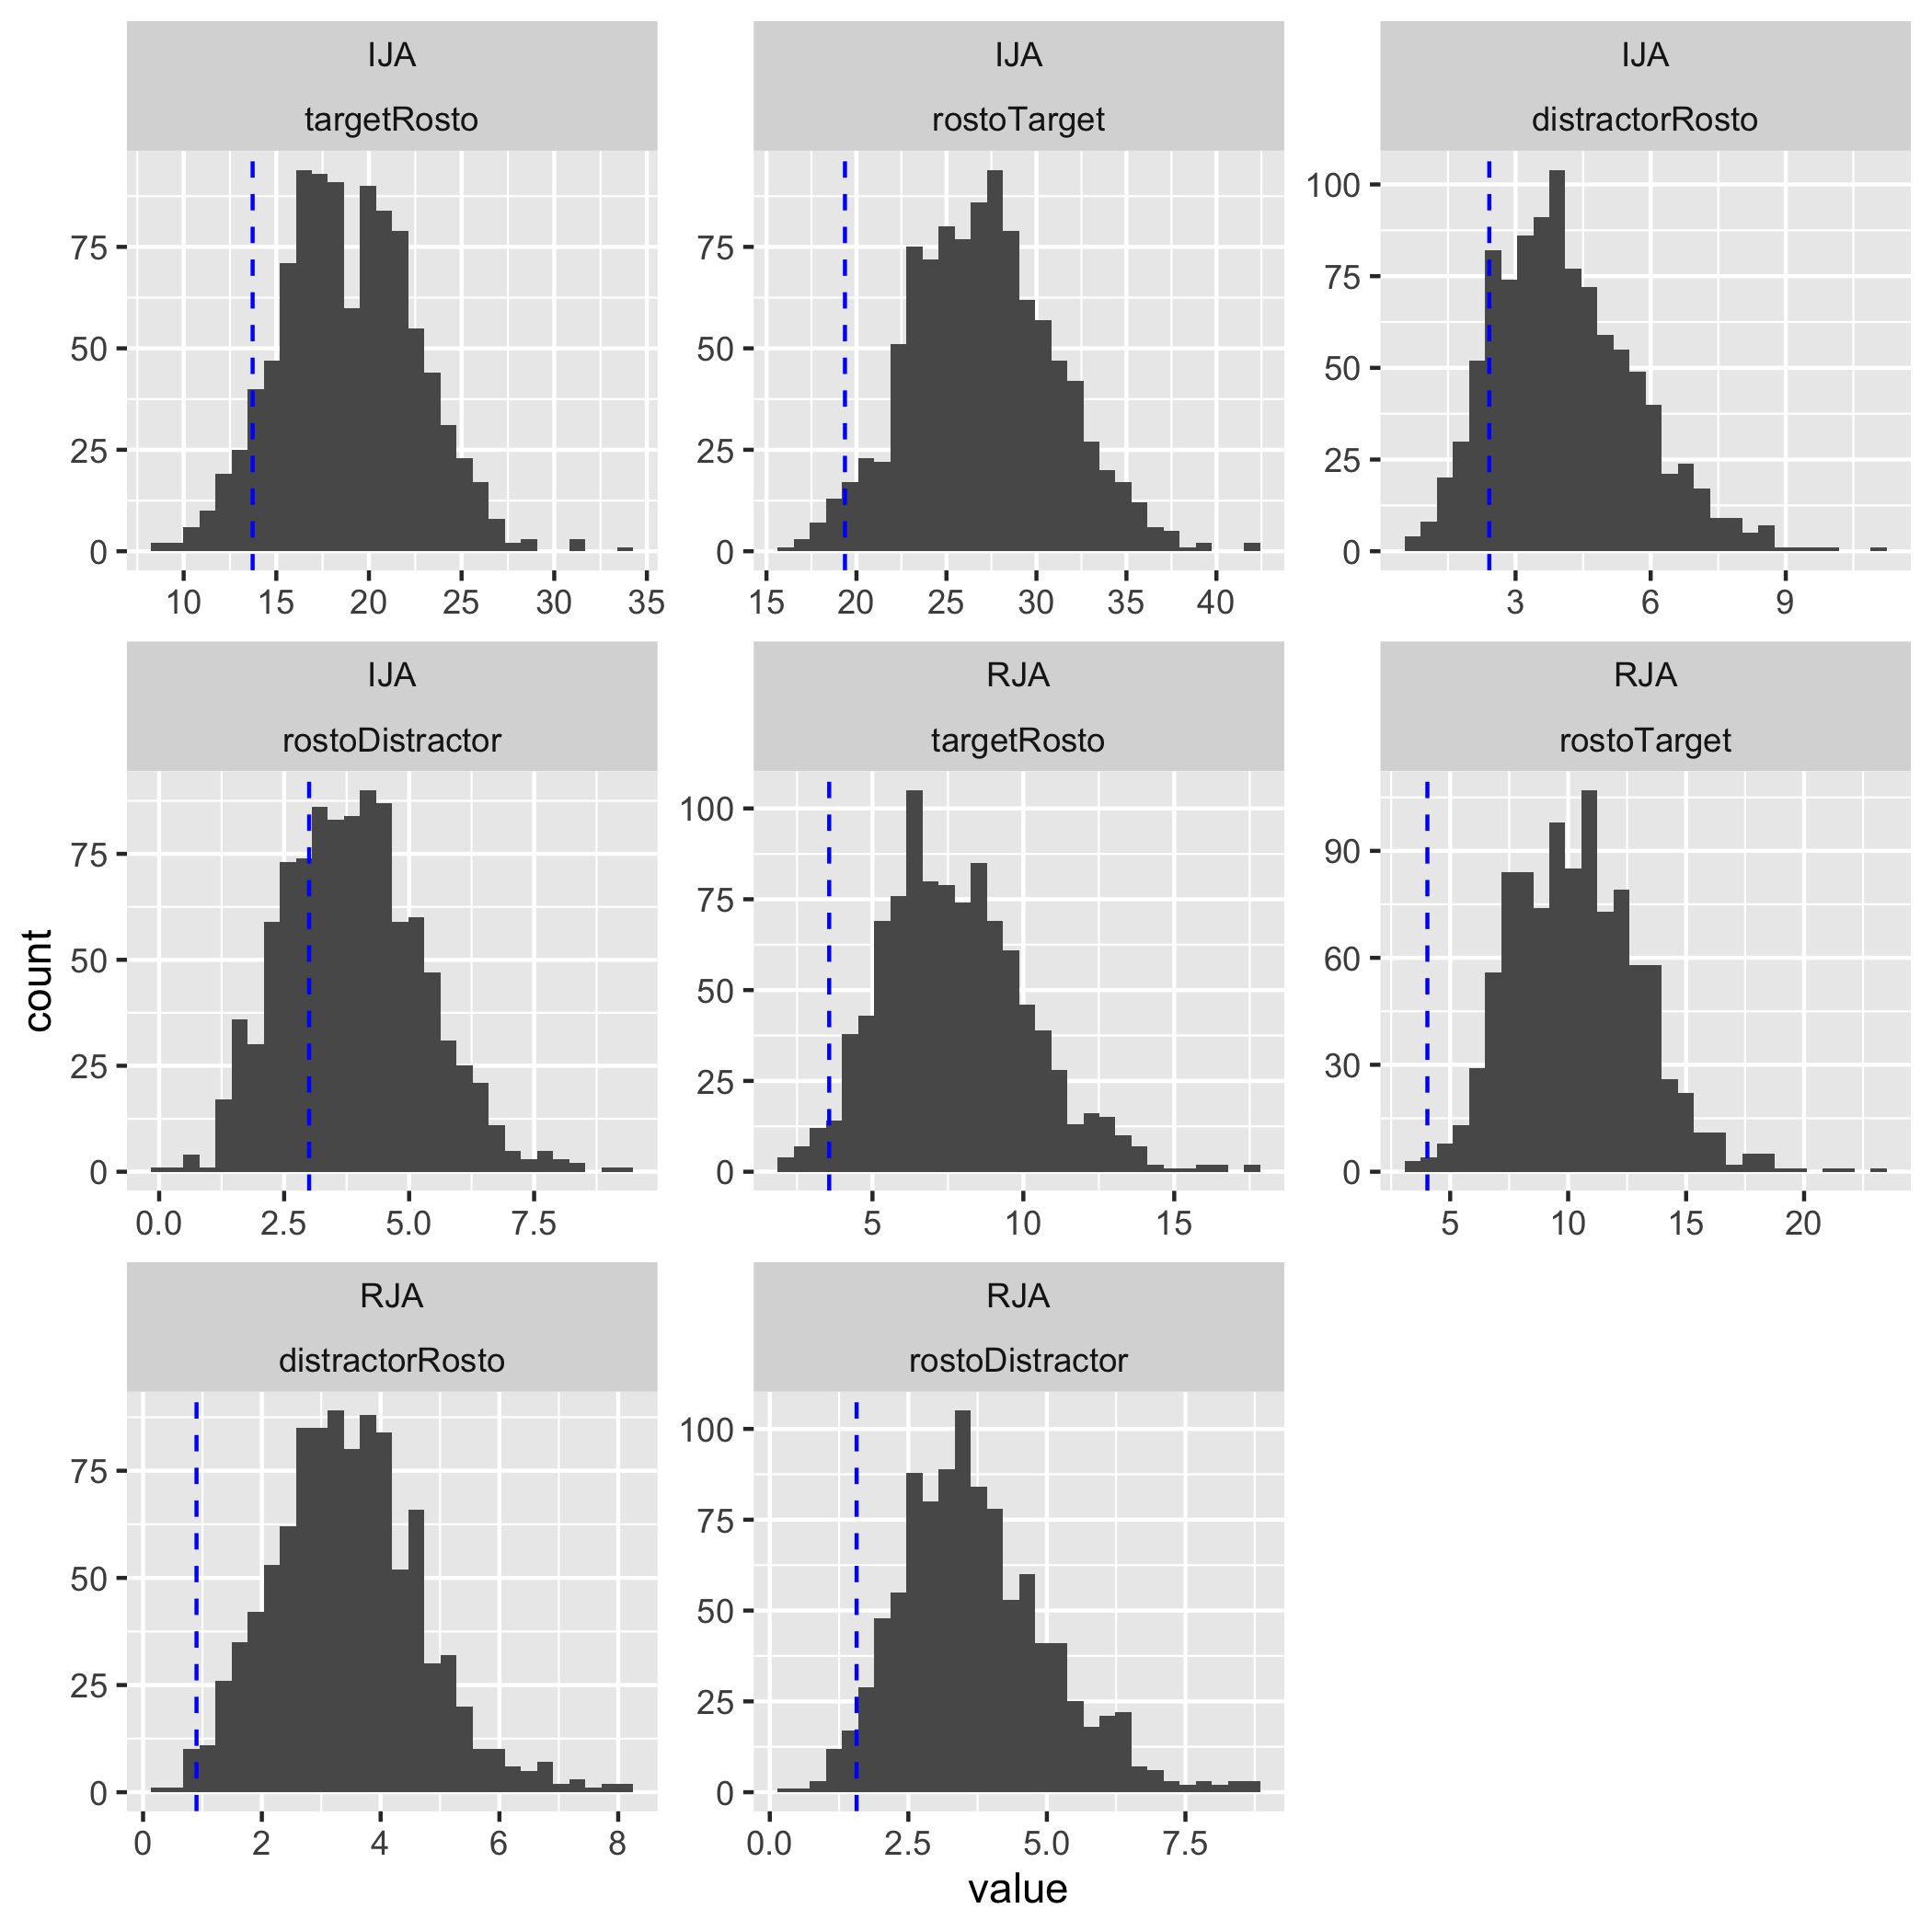
\includegraphics[scale=0.2]{./alternancias.png}}
  \centering
\end{figure}

\subsection{Alternância}

\begin{figure}[H]
  \caption{Média de alternâncias realizadas entre diferentes regiões da tela. Linha pontilhada azul indica o sample de participantes com TEA.}
  \noindent\makebox[\textwidth]{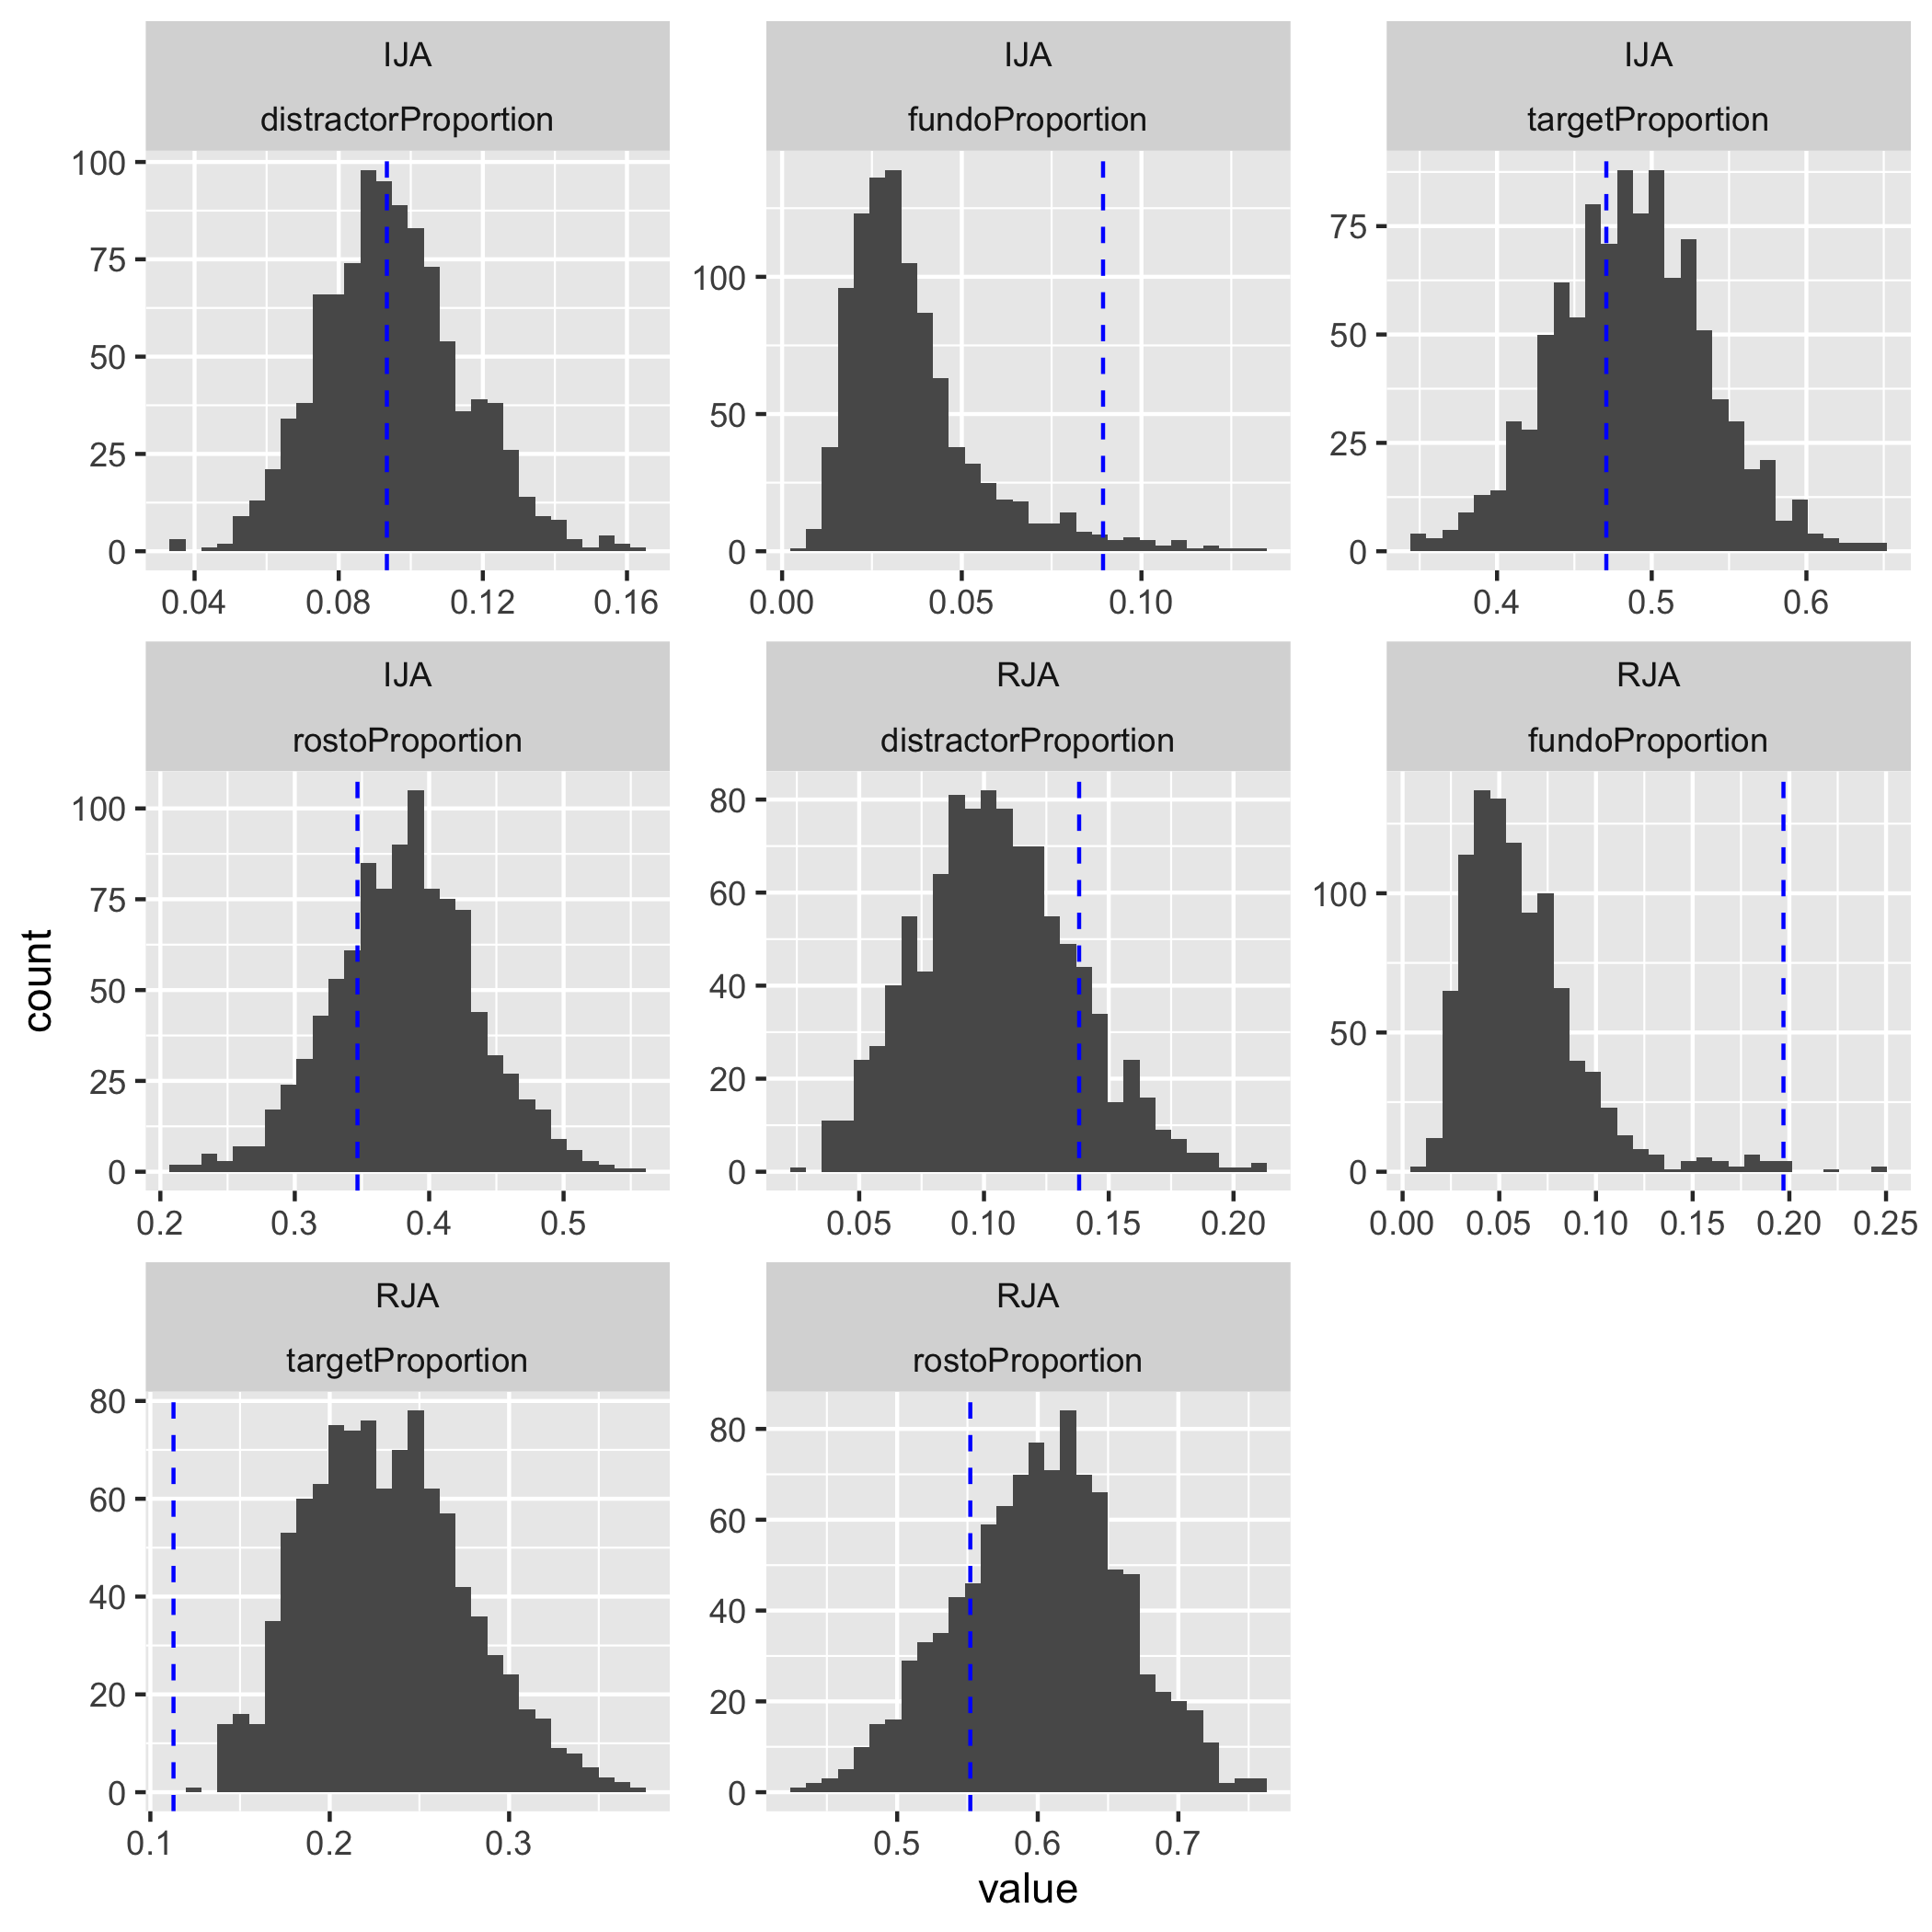
\includegraphics[scale=0.2]{./proportions.png}}
  \centering
\end{figure}

\end{document}

